\noindent There are many solutions for those that are sensorily impaired, helping them complete various tasks, of which autonomous navigation is one of the most complex, ambiguous, and challenging. Presently, the blind may use canes or guide dogs to travel and avoid obstacles; it is not only the fully blind who may rely on these trusted methods, but also the near or farsighted.  In both cases, the system involves guidance in response to sensed information, followed by the person carrying out their course of travel appropriately. The environment itself may correct and guide them, for example, in tight spaces, where they can use railings or rely on memory of certain places where they have a mental picture of its layout. FORWARD seeks to create a universally applicable system based on these realistic cases which can be added as an addendum to any rollator, or even electric wheelchair for that matter. In the medical setting or as physical ailment is compounded onto visual inhibition, motorized and smart solutions are able to show their worth. When the user is less able to navigate on their own, an engineering solution can be formulated in the form of a control system, which informs them about the environment (obstacle detection and identification), and assists their journey while able to warn them about danger and create a smooth navigation feeling while pushing the rollator (avoidance). FORWARD is inherently, all about guidance, navigation, and control, and it borrows aspects from other fields such as robotics, autonomous driving technology, and more. The following section of this document is research of the existing similar products, technologies available, comparison of components to meet design requirements (specified in \ref{sec:req_spec}), and proposed architectures for system integration.\\

\subsection{Existing Products and Projects}
% how have other projects and products used similar strategies to FORWARD?

\noindent There have been numerous efforts made by researchers to develop smart walkers using the available technologies. Perhaps the seminal work in this growing field of research and development is \cite{PAMM}. This group was the first to propose a smart walker project with localization, mobility control, and object avoidance. In the following sections we seek to analyze these technologies and methods in a way that identifies which of such will be most desired for our specific system, taking into consideration many factors, some of which being: cost, attainability, integration complexity, and performance. We also find hardware and software solutions to implement the strategies of design based on \cite{PAMM}. As we will see, these take the form of sensors, processors, and actuators - forming an integrated guidance and control system.\\

%% Toby research here
\subsubsection{Current Walker Sensing Applications}
\noindent Sensing is required to situate and guide the FORWARD walker safely. There are a plethora of technologies and methodologies available today, and we explore some of those.\footnote{\noindent This walker does not employ GPS technology. We are not looking primarily to track the location continuously. This technology has more of a place within the application of health monitoring and emergency alerts. Additionally, we are not using LiDAR environment mapping as many autonomously navigating delivery robots do. This requires what we believe, is an overabundant amount of processing which detracts from the dual nature of the FORWARD user control and guidance} In the smart walker prototype created in \cite{Mostofa}, nine HC-SR04 ultrasonic sensors are arrayed along the front of the walker. Seven face forward, while the remaining two point perpendicularly to the walker motion and opposite to each other. This setup provides a continuous reading of the walker's forward hemisphere with a detection range of 200cm. Our team aims to provide obstacle detection and notification, achieved with a more discrete array of sensors stowed onto the walker frame. We aim to maximize the operational FOV for ultrasonic sensors without requiring a large amount of them. We also anticipate that the introduction of supplemental LiDAR and camera technology will affect the ultrasonic approach. If it happens to be that obstacles have protruding edges, sensors at varying heights along the walker might be required. For instance, a highly directional sensor might miss a railing. For this reason, we also explore camera options later in this section to reinforce and prevent miss cases.\\

\begin{figure}[H]
	\centering
	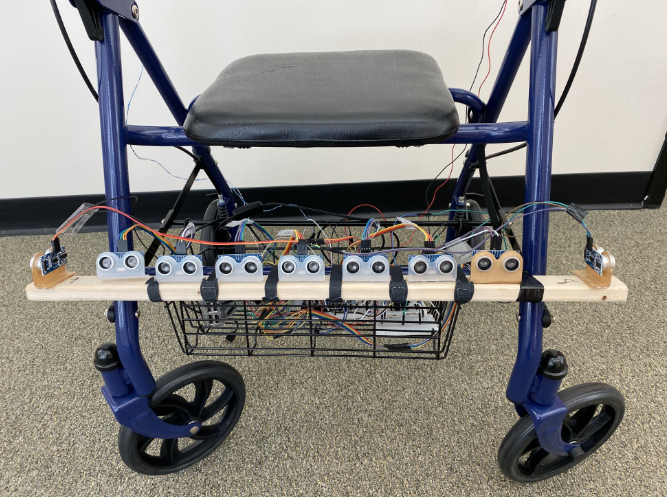
\includegraphics[width=0.5\textwidth]{./Images/mostafa9.png}
	\caption{\label{fig:mostafa9}"Rollator" with nine HC-SR04 sensors \cite{Mostofa}}
\end{figure}

\noindent Robotics are a popular use of LiDAR, often able to achieve feats such as autonomous delivery. However, many researchers have also introduced laser sensing methods and other waves near infrared in order to provide ranging data to mobile systems, which in our case is the walker. A senior design group at Michigan State University expanded on this \cite{mstate}. Their approach to prototyping is beneficial for reference, as they utilized LiDAR Lite and HC-SR04 ultrasonic sensors, all encased with a housing mounted on the crossbar of the handles. This team maintained a discrete add-on to the walker, which is an advantageous feature for the users in their everyday life. It is also from this work that we obtain the incline and decline testing for the prototype, and this is a driving factor for including an IMU on-board the walker. In their topology, the sensors are angled downward so the FOV is more likely to detect ledges or divots; however, in the FORWARD system, we consider reducing this downward tilt to increase detection range, but it is a balance of ideal versus practical.\\

\noindent In \cite{FallDetect}, the group implements one of FORWARD's stretch features with an unorthodox yet clever utilization of LiDAR and sensor fusion. In order to equip the walker with fall detection, both ultrasonic and laser sensors are installed near the footstep bay of the walker. They also add force sensors in the handlebars. The feedback provided by the sensing system is whether the user is walking uprightly. If the user began to fall, the laser sensors would reflect their feet moving out of view, and likely the force sensors would experience more pressure as the user reacted to a slip. Little inspiration is actually drawn from this source, but it is a good illustration of growing interest in smart rollators.\\

%% Morgan and Toby
\subsubsection{Current Walker Stability Applications}
\noindent The byACRE Ultralight Rollator \cite{byACRE} is among a few walkers to feature stability assistance. Initial analysis reveals that this is nothing more than smoothed turning via pneumatic control. The U-STEP Neuro \cite{ustep} is another that features curb lifting, and it features speed control via mechanical configuration of the rolling resistance. The FORWARD group is considering the impact introducing an additional sensor to capture the attitude of the walker and provide data of its speed and turning movements. This technology is explored further in section \ref{sssec:3_2stability}. As we can predict, this sensor will be an inertial measurement unit.\\

%% Matthew Research Here
\subsubsection{Current Computer Vision Object Detection Applications}

% General Synopsis of the current state of research
\noindent There are currently many attempts to develop an image processing/object detection system that, similar to our motivation, seeks to assist the millions of visually impaired people across the globe live normal daily lives. There have already been multiple attempts to exploit the current state of machine learning and AI to to solve this problem. Many of the existing projects implement the YOLO model to develop their object detection algorithms. Many of these projects also implement an audio feedback system to alert the user of any upcoming hazards and important details of such. The following sections detail such research. \\
    
% Project Ref #1
\noindent The project outlined in this paper \cite{CVRef1} aims to provide guidance and navigation to the visually impaired using a user-worn chassis. A notable piece of hardware employed in the project is the high-performance Jetson Nano microcontroller unit (MCU). The Jetson Nano features are further outlined in section \ref{sec:mcu_tech}. \\

\noindent The software aspect of this project is mainly comprised through an object classification system that uses the output of the YOLO5 model to classify the threat level of certain objects. By creating an "area of interest" represented by a 2D and 3D grid, they were able to perform calculations to achieve this. \\

\noindent The figure demonstrating this concept is show below:
				
% Figure 1 in the paper
\begin{figure}[H]
	\centering
	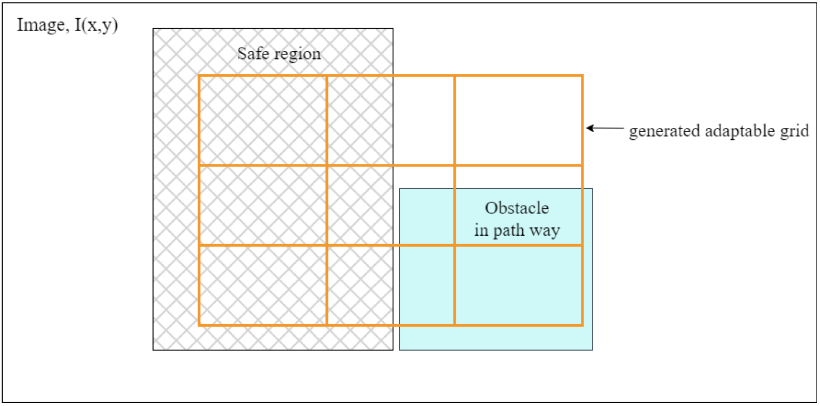
\includegraphics[width=\textwidth]{./Images/Figure1_Grid_Detection.png}
	\caption{\label{fig:Grid-Generatio}2D Grid with Safe Region Generation}
\end{figure}

\noindent Referring to the figure above, once the effective safe region is established, the MCU initiates calculations on the YOLO5 output to deliver accurate guidance to the system. Consequently, this group's approach, which integrates YOLO5 with carefully selected AI/ML-supporting hardware and applied mathematics, ensures precision and reliability for the user. \\

\noindent This project also implemented an audio feedback system. In order to interface to the user regarding the surroundings, there are typically two approaches: auditory and tactile feedback. This group decided to implement auditory feedback with a strategic design to target the use of dorsal and ventral processing, looking to engage the part of the brain created for processing visual cues for spatial awareness.\\

% Project Ref #2
\noindent The project outlined in this paper \cite{CVRef2} sought to design and implement a lightweight FPGA compatible obstacle detection AI model. This project took an approach similar to our scope in choosing a set of objects to train the model on, and look for based on user needs. This project also used a YOLO5 architecture to perform the object identification. This YOLO5 model is suitable for embedded and FPGA devices, allowing for a lightweight AI model that is feasible for these applications. \\


% Project Ref #3
\noindent This project seen in \cite{ESP32CamRef1} seeks to implement a light weight and low cost object detection system using the ESP32 Cam Module. They trained the YOLO3 model on the COCO image data set. They then programmed the board using the ESP32 Cam library. Given this Cam module being connected to an ESP32 chip, they used the WiFi capability to transmit the photos to the laptop. The problem unsolved by this project is that the AI processing is done on a laptop, which has significantly more processing power than our MCU, but proves that this camera is suitable for our purposes of image capturing and transmission. \\

% Project Ref #4
\noindent While the article above primarily addresses the camera solution, it references another article \cite{RealTekCamRef1} that implements a camera solution that can perform the object classification processes as well. The Camera board is the \underline{\textit{Realtek AMB82-Mini IoT AI}} Camera Board, which contains many desired features for our purposes, all of which our outlined in section~\ref{sec:cam_tech} (\textit{Camera Technologies}). In the project referenced, they were able to successfully identify and detect 80 distinct objects of many different categories. They used the Arduino IDE to program the board and then demonstrated functionality. The board transmits the data fully over WiFi as well, which would minimize the overall footprint for our project but minimizing the need for wiring.\\


\subsubsection{Current Audio Feedback Applications/Technologies}
\noindent There are currently many existing projects that exist to implement Bluetooth communication on a microcontroller (MCU). One of these projects \cite{bluetoothSensorProject} implements Bluetooth Low Energy (BLE) to send sensor data to an ESP32 MCU. Bluetooth devices use GATT, which stands for Generic Attributes and it defines a hierarchical data structure of a standard communication protocol. They then used the BLE Universally Unique Identifier (UUID) to identify the sensors specific service. After defining such, they utilized the Bluetooth libraries to create the server, connect the devices, and send out such data. Due to the extensive utilization of Bluetooth in the current state of technology, the pre-existing libraries create easy-to-use interfaces for the programmer to develop efficient Bluetooth communication without many complications. \\


%% Morgan Research Here
\subsubsection{Motor and Steering Applications}
\noindent An electric scooter is a vehicle with similar technology and proportions that we plan to use for our FORWARD walker. Electric scooters also use a controller that is used to communicate between the sensors of the scooter and the motors. Similar to our design, electric scooters also implement safety features that require the actuators to respond given sensor feedback, for example, regenerative braking that responds to the handle brakes and electrical component temperature detection \cite{apollo}. There are even some scooters that employ ultrasonic sensors to detect obstacles and come to a halt in response. An electric scooter that we found to have the capabilities to respond to obstacles uses an Arduino and RKI-1341 Motor driver to control an alarm and braking system \cite{hwang2020}. The braking in this system is operated by a DC motor that pulls the brake lever, whereas in the scooter with regenerative braking, the DC motors go into reverse and slow down the scooter until it comes to a full stop. With this evaluation are examples of several different ways to implement technology for the same purpose on an equivalent device.

